\chapter{CST procedure}
This chapter will detail the steps that should be taken to easily set up a qubit simulation in CST. The determination of the capacitance of the qubit and the electric fields in the structure will be treated separately as the second process is more complex. Both simulations make use of the Frequency Domain Solver. Settings applicable to both processes are the frequency range and the boundaries. 
\begin{itemize}
	\item Under '\textit{Simulation}' click '\textit{Frequency}' and set the desired values.
	\item Again under '\textit{Simulation}' click '\textit{Boundaries}' and set the fields as in figure \ref{fig:Boundaries}
	\item Click '\textit{Open Boundary...}' and under '\textit{Automatic minimum distance to structure}' select '\textit{Fraction of wavelength}' and set to 8. Click '\textit{OK}'.
\end{itemize}

\begin{figure}[h]
	\begin{center}
		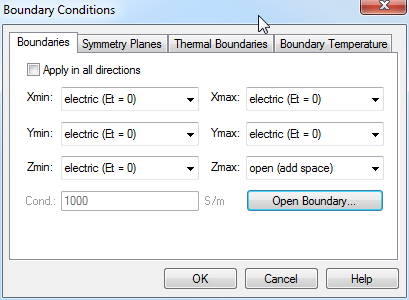
\includegraphics[scale = .7]{Figures/Boundaries}
		\caption{Settings for the boundary conditions of the simulations. All except '\textit{Zmax}' are set to '\textit{electric (Et = 0)}'. '\textit{Zmax}' is set to '\textit{open(add space)}'.}
		\label{fig:Boundaries}
	\end{center}
\end{figure}

\section{The capacitance}
As show in equation \eqref{eq:totalenergy} the capacitance of the structure must be known to calculate the total energy in the qubit. The value of the capacitance converges very quickly as the mesh is refined. This simulation should always include a Discrete Port connected to the capacitor pads.
% 
\subsection{Modeling}
The qubit design can be imported to CST or created in CST itself. Figure \ref{fig:capacitance_basic_setup} shows a qubit designed in CST. It includes two metal pads connected by a discrete port and is surrounded by a metal ground sheet. 
\begin{figure}
	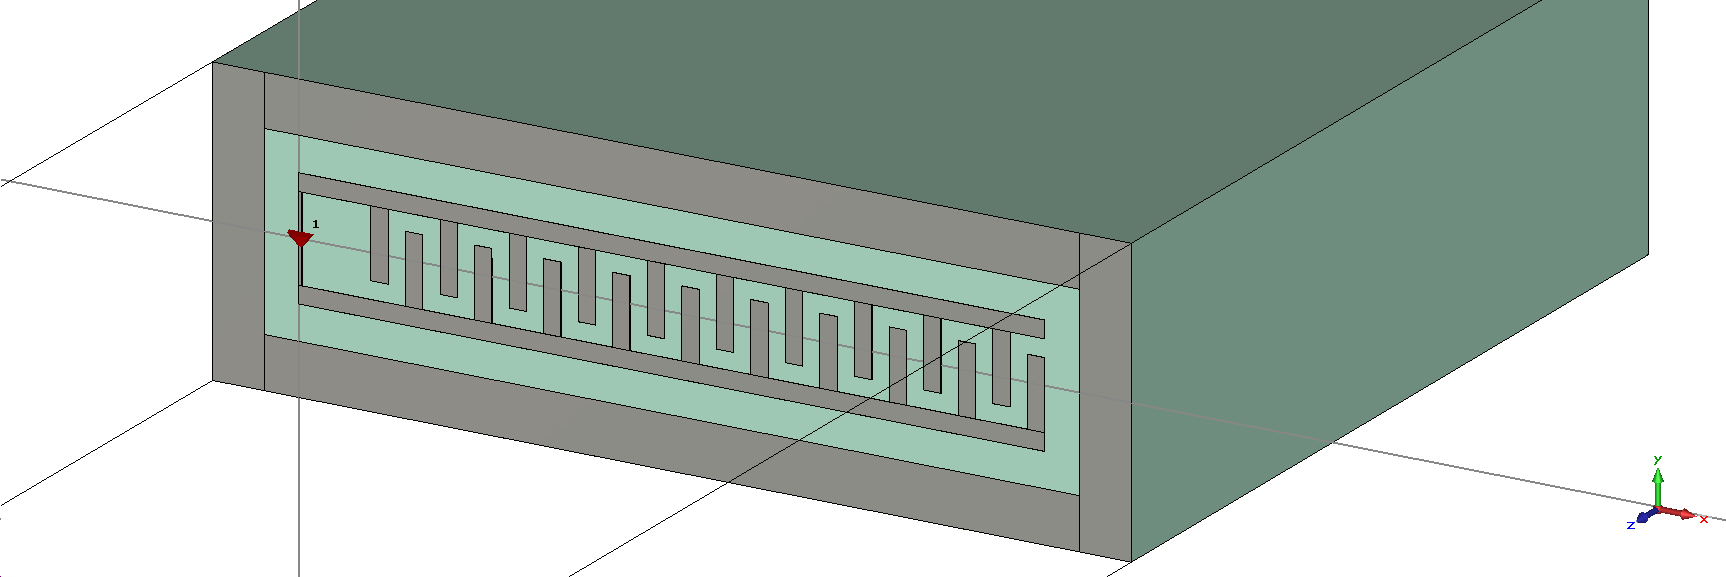
\includegraphics[width=\textwidth]{Figures/capacitance_basic_setup}
	\caption{An example of a qubit design with the substrate in green, the metal parts in grey and the port indicated by the red cone. No lumped element representing the Josephson junction is present in the model.}
	\label{fig:capacitance_basic_setup}
\end{figure}
For the determination of the capacitance, the inductor representing the Josephson junction should be omitted from the simulation.
\subsection{Meshing}
The default settings for the tetrahedral meshing can be used during calculation of the capacitance. This will yield a very rough initial mesh with few mesh elements and will ensure short simulation times.
\subsection{Post processing}
In the post processing templates window, the capacitance of the simulated structure can be retrieved; 
\begin{itemize}
	\item Under '\textit{Post Processing}' select '\textit{Template Based Post Processing}'.
	\item In the pop-up window, in the first selection box choose '\textit{S-Parameters}'.
	\item In the second selection box choose '\textit{Z-parameter}'.
	\item In the pop-up window check the '\textit{C}' option and click '\textit{OK}'.
\end{itemize}
This will yield a 2D graph showing the capacitance of the structure as a function of frequency. \\
Now include a second template;
\begin{itemize}
	\item In the first selection box choose '\textit{General 1D}'.
	\item In the second selection box choose '\textit{0D or 1D Results from 1D Result (Rescale, Derivation, etc)}'.
	\item In the pop-up window select '\textit{y at given x}' and set '\textit{Evaluate at x =}' to the desired frequency. Click '\textit{OK}'.
\end{itemize}
After simulation, the result should be a single value of the capacitance at the required frequency.

\subsection{Simulation setup}
To ensure convergence of the capacitance, results from the post processing templates can be used as targets for the simulation;
\begin{itemize}
	\item Under '\textit{Simulation}' choose '\textit{Setup Solver}'.
	\item Under '\textit{Adaptive mesh refinement}' make sure the '\textit{Adaptive tertrahedral mesh refninement}' is checked and click '\textit{Properties}'.
	\item In the pop-up window under '\textit{Number of passes}' set the maximum to at least 8.
	\item Under '\textit{Check after broadband calculation:}' mark the '\textit{OD result Template...}' as active and select the 0D result of the capacitance from the post processing template above. 
	\item Set the required Treshold and Checks as desired and click '\textit{OK}'.
\end{itemize}
This will ensure the simulation keeps refining the simulation until your demands on accuracy are met or until maximum amount of mesh refinement passes is reached. After every mesh refinement pass the results are updated and can be checked. In the Navigation Tree click '\textit{Tables}' \(\rightarrow\) '\textit{0D Results}' \(\rightarrow\) '\textit{C1,1\_0D\_yAtX}'. The first result will be viewable once the first pass of the simulation is completed. When the simulation is finished the capacitance of the structure can extracted from the plot. An example is given in figure \ref{fig:capacitanceplot}.

\begin{figure}
	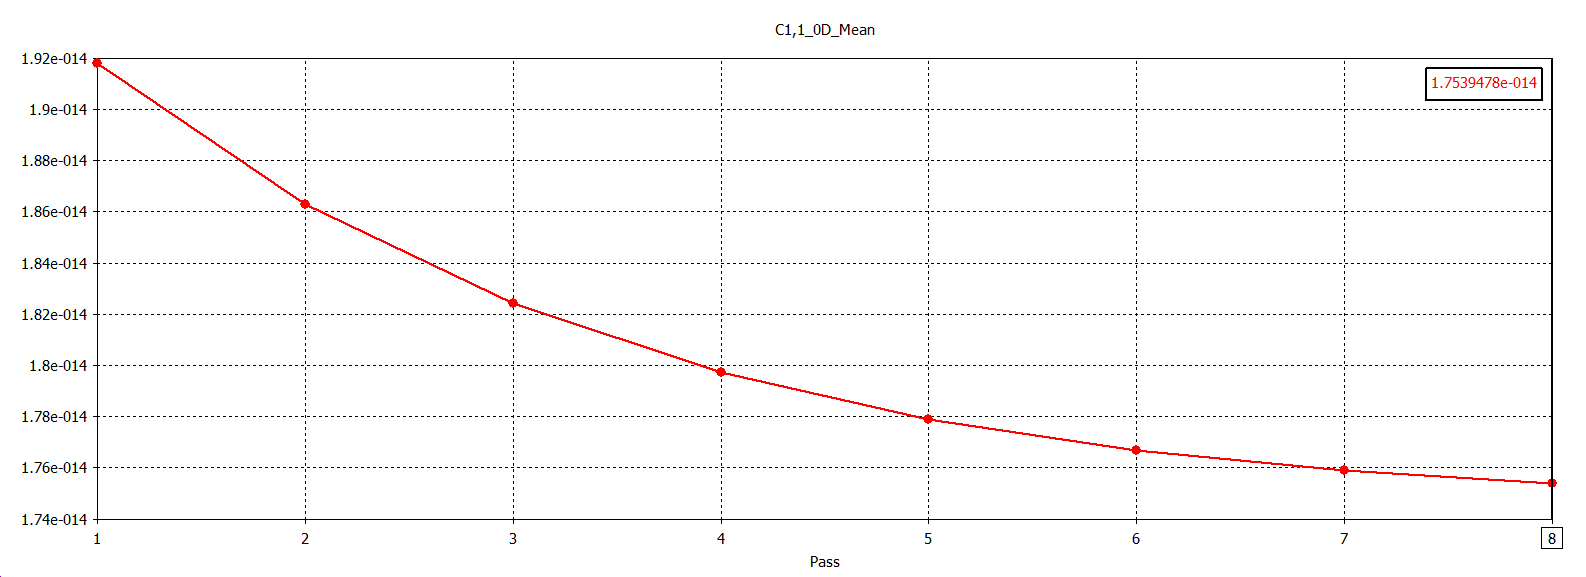
\includegraphics[width=\textwidth]{Figures/capacitanceplot}
	\caption{An example of the data retrieved on the capacitance of a qubit design. On the y-axis is the capacitance in Farad. On the x-axis is the number of mesh refinement passes. Highlighted is the value of the capacitance after 8 passes.}
	\label{fig:capacitanceplot}
\end{figure}

\section{The electric field}
Now that the capacitance of the structure is known the more extensive simulation of the electric field can be set up.
\subsection{Modeling}
Using equation \eqref{eq:impedance} the inductance needed to reach a certain resonance frequency can be calculated. 

\begin{equation}\label{eq:impedance}
L = \frac{1}{(2\pi)^{2}f_{0}^{2}C}
\end{equation}
Where \(f_{0}\) is the required frequency and \(C\) is the capacitance.\\
Now to include such an inductor;
\begin{itemize}
	\item In the simulation menu add a '\textit{Lumped element}'.
	\item Set the element '\textit{Type}' to be '\textit{RLC parallel}'
	\item Set the value of the inductance as calculated and leave the other values at zero.
	\item Make sure the '\textit{Monitor voltage and current}' is checked.
	\item Set the location as desired or use picked points.
\end{itemize}

Next, to ensure a fine initial mesh, the edges on the side of the pads are rounded. In order to make this possible each pad must be a single object. To achieve this the '\textit{Boolean}' operation can be used to combine multiple object into one;

\begin{itemize}
	\item In the Navigation Tree, under '\textit{Components}' select all objects pertaining to one pad.
	\item Under '\textit{Modeling}' click the '\textit{Boolean operator}'.
\end{itemize}
Now that the pad consists of a single object, its side edges can be rounded.
\begin{itemize}
	\item Under '\textit{Modeling}' click '\textit{Picks}' and choose '\textit{Pick Edge Chain}' (or use Shift+E)
	\item Select all the edges laying in the \(xy\)-plane.
\end{itemize}
Figure \ref{fig:blending1} show what the selection should look like. Once the right edges are selected they can be rounded;
\begin{itemize}
	\item Under '\textit{Modeling}' click '\textit{Blend}'.
	\item Set the '\textit{radius}' to be half the height of the pad. 
\end{itemize}
The result should be as in figure \ref{fig:blending3}.


%\begin{figure}%
%	\centering
%	\subfloat[label 1]{{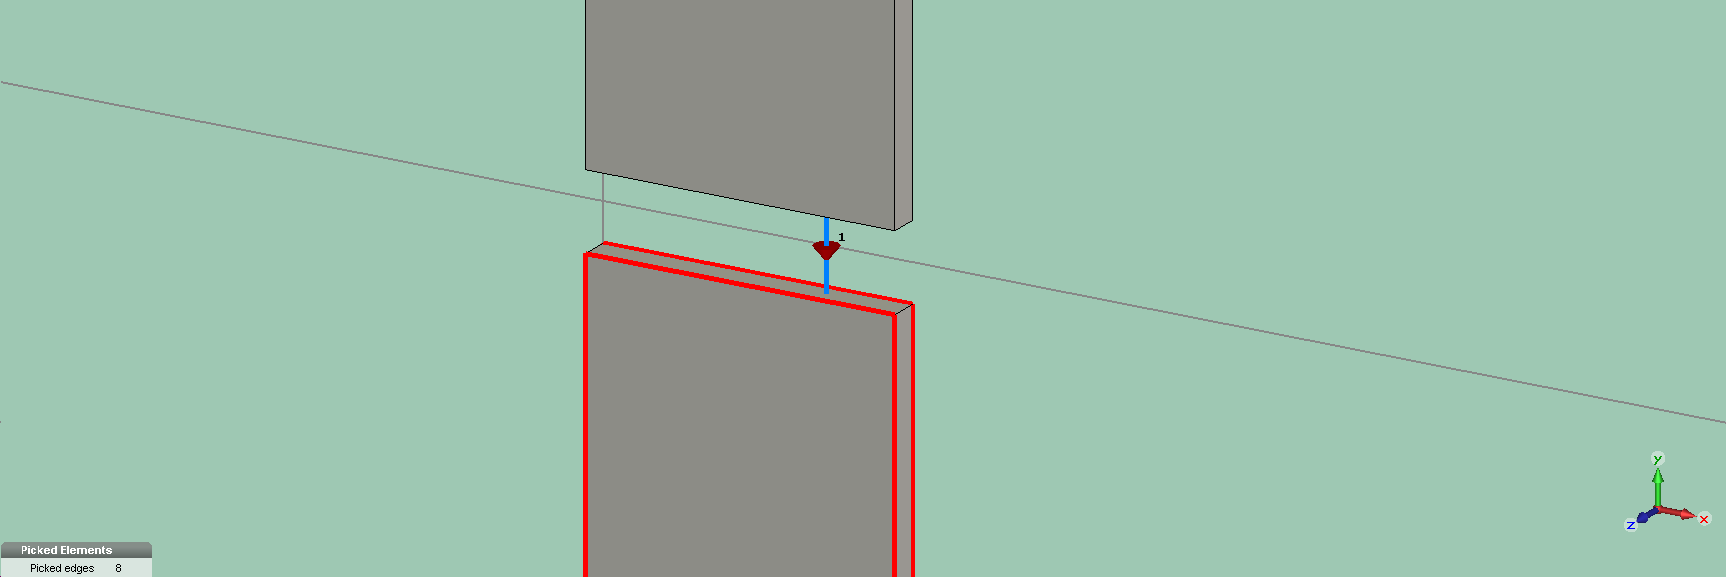
\includegraphics[width=5cm]{Figures/blending1} }}%
%	\qquad
%	\subfloat[label 2]{{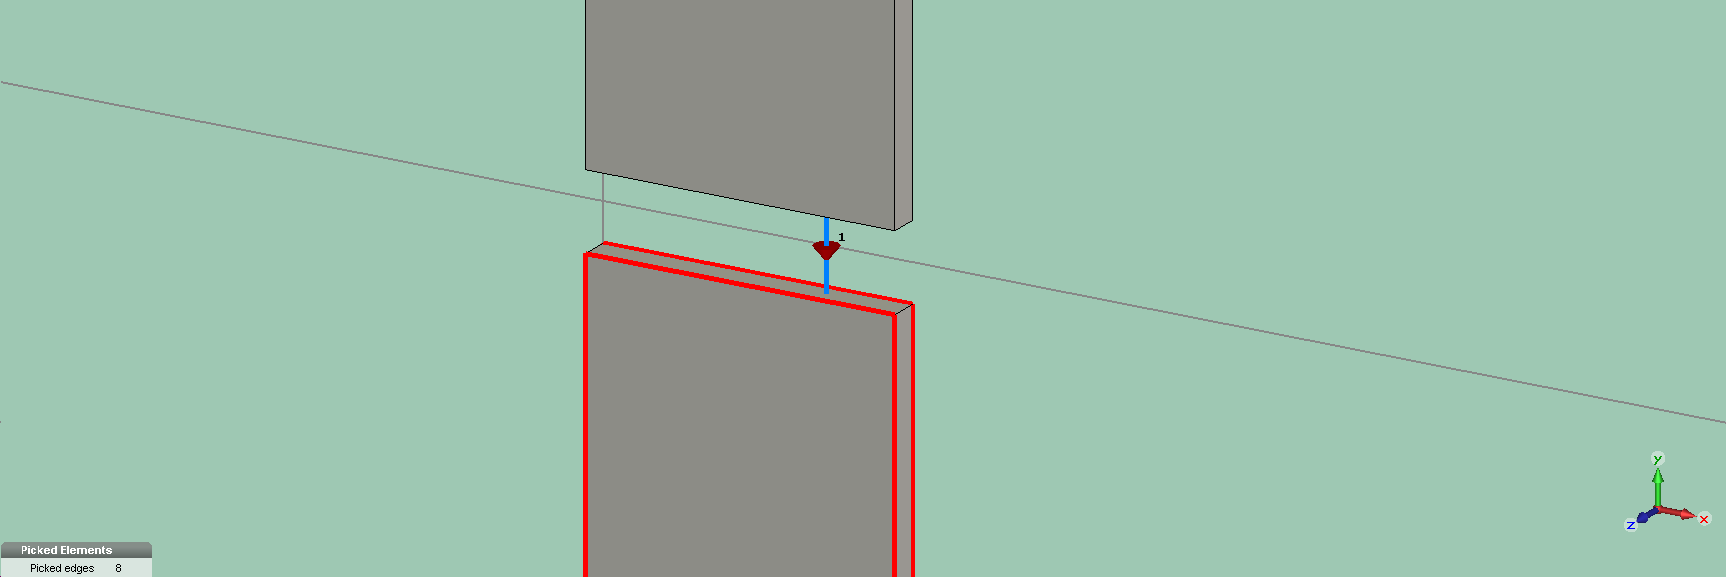
\includegraphics[width=5cm]{Figures/blending1} }}%
%	\caption{2 Figures side by side}%
%	\label{fig:example}%
%\end{figure}
%\begin{figure}[h]
%%	\begin{center}
%		\begin{subfigure}[b]{0.4\textwidth}
%		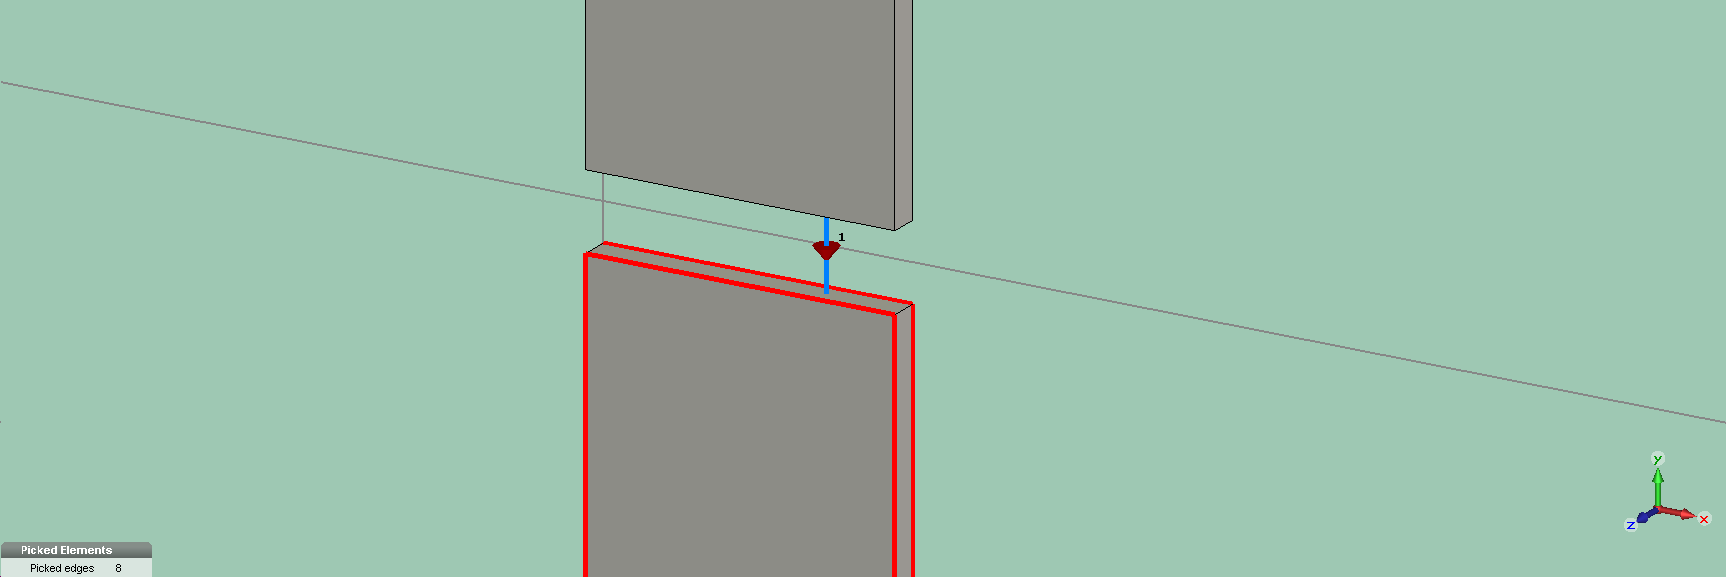
\includegraphics[width = 0.3\textwidth]{Figures/blending1}
%		\end{subfigure}
%		\begin{subfigure}[b]{0.4\textwidth}
%		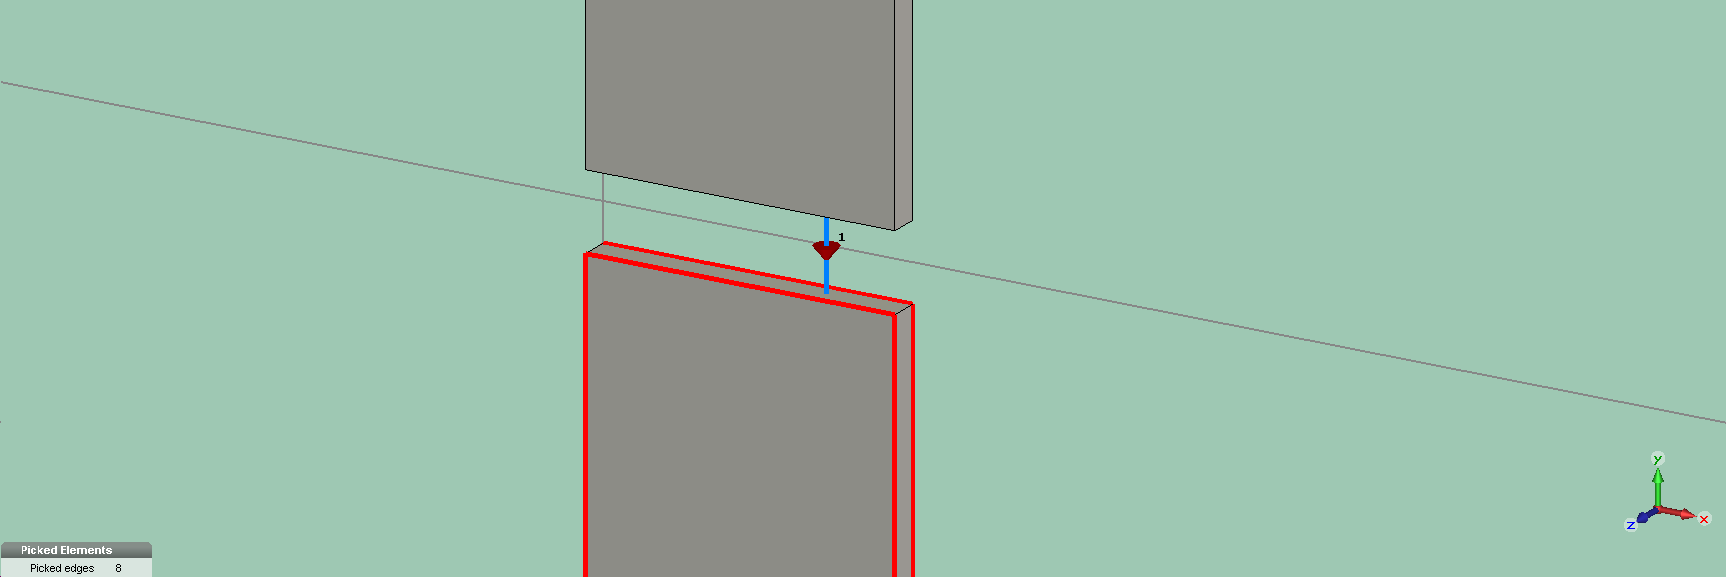
\includegraphics[width = 0.3\textwidth]{Figures/blending1}
%		\caption{A selection of two Edge Chains in red. One at the level of the substrate and another at the level of the top of the pad.}
%		\label{fig:blending1}
%%	\end{center}
%\end{figure}
\begin{figure}[h]
  	\begin{center}
 		
 		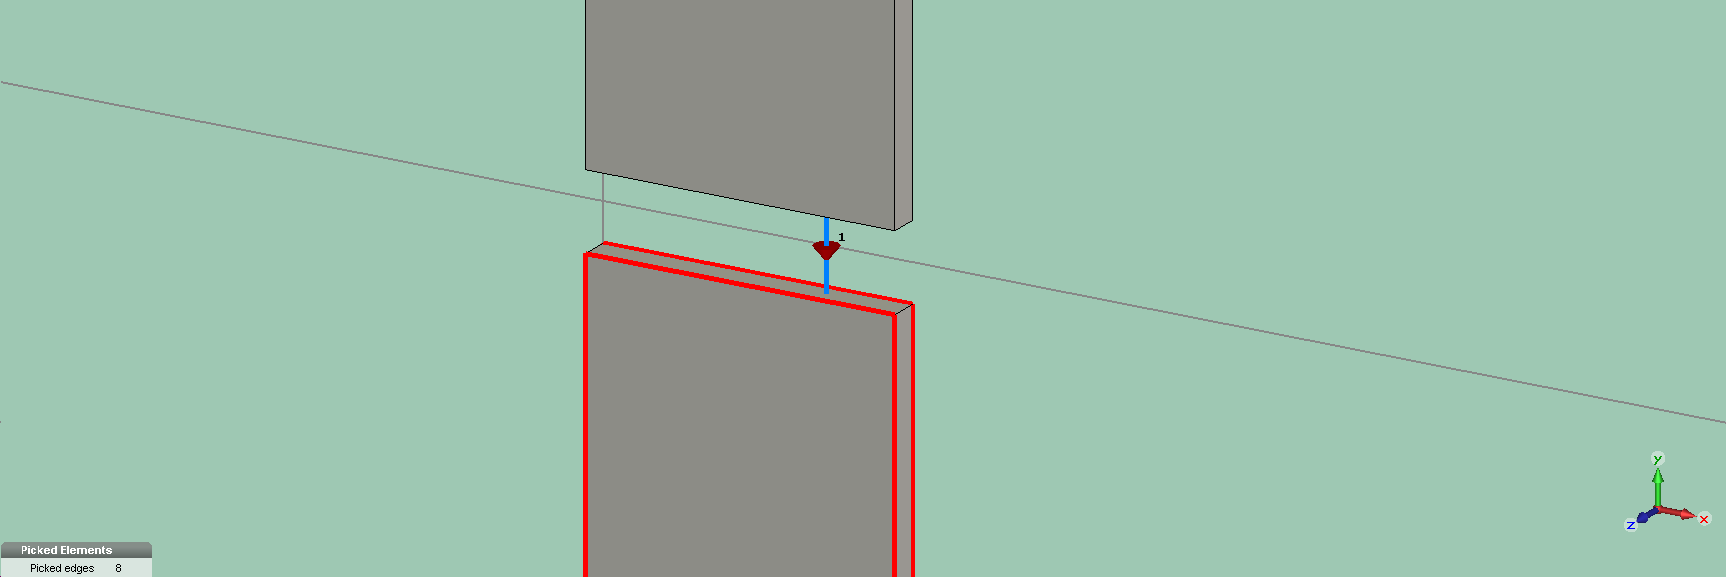
\includegraphics[width = 0.3\textwidth]{Figures/blending1}
 		\caption{A selection of two Edge Chains in red. One at the level of the substrate and another at the level of the top of the pad.}
 		\label{fig:blending1}
  	\end{center}
 \end{figure}
\subsection{Meshing}
In order to obtain a fine initial mesh the \textit{Global mesh properties} can be changed;
\begin{itemize}
	\item Under '\textit{Simulation}' click '\textit{Global mesh properties}'.
	\item In the pop-up window click '\textit{Specials}'.
	\item Under the '\textit{Mesh Control}'-tab set '\textit{Smooth mesh with equilibrate ratio}' to \(1.15\).
	\item Set '\textit{Normal tolerance}' to \(1\) degree.
	\item \textbf{Uncheck} the '\textit{Anistropic curvature refinement}'.  
\end{itemize}
See figure \ref{fig:MeshProperties} for the settings.
\begin{figure}
	\begin{center}
		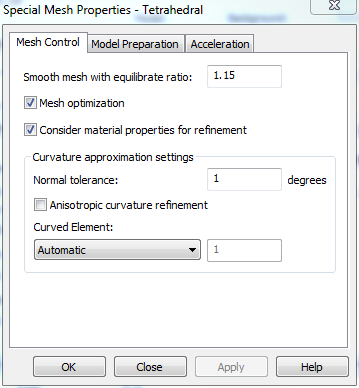
\includegraphics[scale = .6]{Figures/MeshProperties}
		\caption{The required settings for the Mesh Properties. The Anistropic curvature refinement must be unchecked!}
		\label{fig:MeshProperties}
	\end{center}
\end{figure}

\subsection{Simulation setup}
To be able to view and save field data, include a field monitor;
\begin{itemize}
	\item Under '\textit{Simulation}' click '\textit{Field Monitor}'.
	\item In the pop-up window select the e-field monitor and choose a frequency.
	\item Click '\textit{OK}', the monitor should be visible in the Navigation Tree.
\end{itemize}

\subsection{Exporting data}
To calculate the participation ratio the simulated electric field is exported as an ASCII file. In order to separate data pertaining to different lossy layers the data for the field on the Pads, Substrate and Ground can be exported separately. 
\begin{itemize}
	\item In the Navigation Tree under '\textit{Components}' hide all objects until only the Pads are visible.
	\item Again in the Navigation Tree open the '\textit{2D Results}' folder.
	\item Select the '\textit{Abs}' component of the '\textit{E-Field}'.
	\item Under '\textit{Post Processing}' click '\textit{Import/Export}' and click '\textit{Export as ASCII file}'. 
\end{itemize}
Repeat these steps for the Substrate and Ground.